\documentclass{beamer}

\usepackage[utf8]{inputenc}           % Paquetes para idioma
\usepackage[spanish,es-tabla]{babel}
\usepackage{color}                    % Para cambiar el color de las letras
\usepackage{pagecolor}                % Para cambiar el color de las pagina
\usepackage{graphicx}                 % Para incluir graficos
\usepackage{placeins}                 % para evitar que se descuadre el texto con respecto a las imagenes
\usepackage{wrapfig}                  % Para texto alrededor de las figuras
\graphicspath{{img/}}                 % Todas las imágenes se cargan del subdirectorio 'img' por defecto.
\usepackage{amsmath}                  % Para más símbolos matemáticos
\usepackage{amsthm}                   % Para más símbolos matemáticos
\usepackage{amssymb}                  % Para incluir algunos simbolos matematicos
\usepackage{marvosym}                 % Para incluir simbolo de Euro
\usepackage{pifont}                   % Para incluir simbolos ding
\usepackage[T1]{fontenc}              % Para Codificación tipo 1 del archivo.
\usepackage{enumerate}                %Para trabajar con listas enumeradas
\usepackage{lipsum}                   % Para texto Lorem Ipsum
\usepackage{enumitem}                 % Paquete que permite dar configuración adicional a los espacios entre itemize, enumerate etc, ( listas )
\usepackage{tabularx}                 % Para hacer tablas 
\usepackage{booktabs}                 % para opciones adicionales
\usepackage{array} 
\usepackage{multirow}                 % Permite construir tablas en la que las celdas ocupan varias filas 
\usepackage{dcolumn}                  % Para dividir columna por una diagonal
\usepackage{colortbl}                 % PAra usar colores en tablas
\usepackage{parskip}                  % Descomentar para que los parrafos no comiencen con sangria. y espacio interlineado
\usepackage{tikz}                     % Para framezoom con circulos
\usetikzlibrary{spy}                  % Para framezoom con circulos
\setbeamercovered{transparent}        % para que los items se vean en transparente antes de ser seleccioandos
\setbeamertemplate{navigation symbols}{}

\usetheme{Madrid}
\usecolortheme{seahorse}  % albatross,beetle,crane,dove,fly,seagull,whale,seahorse,lily,orchid

% \beamersetaveragebackground{red}    %Para definir el color de fondo
\useinnertheme[shadow]{rounded}       % Para que bullets sean circulares
% \useinnertheme{rectangles}          % Bullets son cuadrados

\setbeamercolor{postit}{bg=yellow!30!white} % Para un bloque diferente amarillo

%\usepackage{media9}
\usepackage{multimedia}

% \logo{
\includegraphics[width=0.65cm]{logo}} % logo aparece en todas las paginas
\titlegraphic{ 
\includegraphics[width=1cm]{logo} } % aparece solo en la primera pagina y centrado
% \usebackgroundtemplate{
\includegraphics[width=\paperwidth]{1.jpg}} % Agrega 1.jpg como background

% \setbeamertemplate{background}{     % Logo centrado y con opacidad de 0.1
%   \tikz[overlay,remember picture]\node[opacity=0.1] at (current page.center){
\includegraphics[width=3cm]{logo}};
% }

\title[Título corto]{Título largo}
\subtitle{Subtitulo} 
\author{dasesu}
\institute{Nombre de la institución}
\date{15 de enero de 2020}

\begin{document}
% ----------------------------------------- %

  % Pagina 1: Esta corresponde a la portada
  \begin{frame}
  \titlepage % titulo de la primera pagina
  \end{frame}

% ----------------------------------------- %

  % Pagina 2: 
  \begin{frame}
    \frametitle{Tabla de Contenido} % Coloca el título (método 1)
    \tableofcontents % índice de contenido
  \end{frame}

% ----------------------------------------- %

  % Pagina 3:
  \section{Sección 1}  % definiendo secciones y subsecciones: 
                      % esto es lo que en realidad se ve en el índice
  \begin{frame}{Otra forma de colocar título} % Coloca el titulo (método 2)
    \framesubtitle{Subtítulo 1} % Subtitulo

    Un poco de contenido % contenido

  \end{frame}

% ----------------------------------------- %

  % Pagina 4:
  \section{Ejemplo de sección: itemize} % definiendo una sub sección
  \begin{frame}
    \frametitle{Ejemplo de listas}
    \framesubtitle{Usando itemize}
    \begin{itemize}
       \item Primer elemento
       \item Segundo elemento
       \item ...
       \item N-esimo elemento
    \end{itemize}
  \end{frame}

% ----------------------------------------- %

  % Pagina 5:
  \section{Ejemplo de sección: enumerate} % definiendo una subsección
  \begin{frame}
    \frametitle{Ejemplo de listas}
    \framesubtitle{Usando enumerate}
    \begin{enumerate}
      \item Primer elemento
      \item Segundo elemento
      \item N-esimo elemento
    \end{enumerate}
  \end{frame}

% ----------------------------------------- %

  \section{Ejemplo de sección: Overlays} % definiendo una subsección
  \begin{frame}
    \frametitle{Overlays básicos} % en cada parte de nuestra lista van apareciendo de uno en uno.
    \framesubtitle{Opcion: Aparecen todos a la vez}
    \begin{enumerate} % No se esta aplicando ninguna instruccion
      \item Primer elemento
      \item Segundo elemento
    \end{enumerate}
  \end{frame}

% ----------------------------------------- %

  \subsection{Ejemplo de subsección: Overlays} % definiendo una subsección
  \begin{frame}
    \frametitle{Overlays básicos} % en cada parte de nuestra lista van apareciendo de uno en uno.
    \framesubtitle{Opcion:<+->}
    \begin{itemize}
      \item<+-> Primer elemento
      \item<+-> Segundo elemento
      \item<+-> Tercer elemento
    \end{itemize}
  \end{frame}

% ----------------------------------------- %

  \subsection{Ejemplo de subsección: Overlays} % definiendo una subsección
  \begin{frame}
    \frametitle{Overlays} % en cada parte de nuestra lista van apareciendo de uno en uno.
    \framesubtitle{Opcion:<+-> en el Itemize}
    \begin{itemize}
      \item Primer elemento (desde el item)
      \item Segundo elemento
      \item Tercer elemento
    \end{itemize}
  \end{frame}

% ----------------------------------------- %

  \subsection{Ejemplo de sub Sección: Overlays} % definiendo una subsección
  \begin{frame}
    \frametitle{Overlays básicos} % en cada parte de nuestra lista van apareciendo de uno en uno.
    \framesubtitle{Opción: <+-> en explicito}
    \begin{itemize}
      \item<1> Aparece en la primera únicamente
      \item<2-> Aparece desde la segunda en adelante
      \item<-3> Aparece en la primera, la segunda y la tercera
      \item<2-4,6> Aparece desde la segunda hasta la cuarta y luego vuelve a aparecer en la sexta
    \end{itemize}
  \end{frame}

% ----------------------------------------- %

  \begin{frame}
    \frametitle{Overlays básicos} % en cada parte de nuestra lista van apareciendo de uno en uno.
    \framesubtitle{Opción: <+-> en explicito}
    \begin{itemize}
      \item \textbf<1> {Se resalta en negrita solo la primera}
      \item \textbf<2> {Se resalta en negrita la segunda}
      \item \textbf<3> {Se resalta en negrita la tercera} 
      \item \textbf<4> {Se resalta en negrita la cuarta}
    \end{itemize}
  \end{frame}

% ----------------------------------------- %

  \begin{frame}
    \frametitle{Overlays básicos} % en cada parte de nuestra lista van apareciendo de uno en uno.
    \framesubtitle{Opción: <+-> en explicito}
    \begin{itemize}
      \item<1-> \textbf<1> {Se resalta en negrita solo la primera}
      \item<2-> \textbf<2> {Se resalta en negrita la segunda}
      \item<3-> \textbf<3> {Se resalta en negrita la tercera} 
      \item<4-> \textbf<4> {Se resalta en negrita la cuarta}
    \end{itemize}
  \end{frame}

% ----------------------------------------- %

  \begin{frame}
    \frametitle{Overlays básicos} % en cada parte de nuestra lista van apareciendo de uno en uno.
    \framesubtitle{Opción: }
    \begin{itemize}
      \item <+-> desde la primera o actual en adelante con la instruccion <+->
      \item <.-> se repite el valor anterior con el "."
    \end{itemize}
  \end{frame}

% ----------------------------------------- %

  \begin{frame}
    \frametitle{Overlays básicos} % en cada parte de nuestra lista van apareciendo de uno en uno.
    \framesubtitle{Opción: }
    \begin{itemize}
      \item<1-|alert@1> Tiene efecto desde la primera en adelante pero alert en la primera nada mas
      \item<2-|alert@2> Tiene efecto desde la segunda en adelante pero alert en la segunda nada mas
      \item<3-|alert@3> Tiene efecto desde la tercera en adelante pero alert en la tercera nada mas
    \end{itemize}
  \end{frame}

% ----------------------------------------- %

  \begin{frame}
    \frametitle{Un bloque natural} 
    \begin{block}{Título del bloque}
    \begin{itemize}
      \item Elemento
      \item Otro elemento
    \end{itemize}
    \end{block}
  \end{frame}

% ----------------------------------------- %

   \begin{frame}
   \frametitle{Mas ejemplos de bloques} 
   \begin{exampleblock}{Título del bloque}<+->
      \begin{itemize}
      \item Un item
      \item Otro item
      \item Otro item más
      \end{itemize}
   \end{exampleblock}

   \begin{exampleblock}{Título del bloque}<+->
      \begin{itemize}
      \item<+-> Un item
      \item<+-> Otro item
      \item<+-> Otro item más
      \end{itemize}
   \end{exampleblock}
   \end{frame}

% ----------------------------------------- %

  \begin{frame}
    \frametitle{Un blocque de Alerta} 
    \begin{alertblock}{Título del bloque}
      \begin{itemize}
        \item Un item
        \item Otro item
        \item Otro item más
      \end{itemize}
    \end{alertblock}
  \end{frame}

% ----------------------------------------- %

  \begin{frame}
    \frametitle{Un bloque de Amarillo} 
    \framesubtitle{Subtitulo}
    \begin{beamercolorbox}{postit}
      Texto dentro de contenedor amarillo
    \end{beamercolorbox}
  \end{frame}

% ----------------------------------------- %

   \begin{frame}
   \frametitle{Opciones del entorno beamerbox} 
      \begin{block}{Título del bloque}
        wd={Anchura} dp={Profundidad} ht={Altura} (Dimensiones)\\
        left right center (alineaciòn)\\
        sep=Distancia (Separación entre texto y marco de la caja)\\
        rounded=true (false)(Dibujalasesquinasredondeadas) \\
        shadow=true (false)(Colo caunasombra)
      \end{block}
      \begin{beamercolorbox}[sep=3mm]{postit}
        Texto 1
      \end{beamercolorbox}
      \begin{beamercolorbox}[wd=3cm,sep=3mm]{postit}
        Texto 2
      \end{beamercolorbox}
      \begin{beamercolorbox}[wd={4cm},sep=1mm,center,rounded=true,shadow=true]{postit}
        Texto 3
      \end{beamercolorbox}
   \end{frame}

% ----------------------------------------- %

  % EJEMPLO DE COLUMNAS 
  \begin{frame}
  \frametitle{Dos columnas}
  \begin{columns}

    \column{0.45\textwidth}
    \begin{block}{Título del bloque}
      Esto es contenido de la primera columna.
      $$E=mc^2$$
    \end{block}
    \begin{itemize}
      \item Primer elemento
      \item Segundo elemento  
    \end{itemize}   

    \column{0.45\textwidth}
    Esto se muestra en la segunda columna
    \begin{exampleblock}{Título del bloque}
      Este texto y bloque aparecen en la segunda columna.
      $$ y=mx+b $$
    \end{exampleblock}

  \end{columns}
  \end{frame}

% ----------------------------------------- %

  \begin{frame}
  \begin{columns}
    \column{0.45\textwidth} % Ancho de la columna
    \begin{block}{Resultados}
      \begin{itemize}
      \item<1-> Comentario a la Figura 1
      \item<2-> Comentario a la Figura 2
      \item<3-> Comentario a la Figura 3
      \end{itemize}
    \end{block}

    \column{0.45\textwidth}
    \begin{center}
      \only<1> {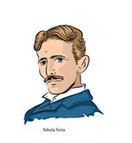
\includegraphics[height=3.5cm]{p1.png}}%
      \only<2> {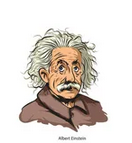
\includegraphics[height=3.5cm]{p2.png}}%
      \only<3> {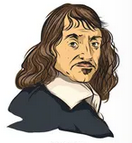
\includegraphics[height=3.5cm]{p3.png}}%
    \end{center}
  \end{columns}
  \end{frame}

% ----------------------------------------- %

  \begin{frame}{Framezoom}
  \hypersetup{linkbordercolor={red!70!black}}
  \framezoom<1><2>[border=2](8.3cm,0.3cm)(1cm,1cm) % Primeras coordenadas son del punto
                                                   % izquierdo superior, las siguientes
                                                   % cuanto me desplazo a partir de alli,
                                                   % por ejem,plo (1,2)(1,1) va a colocar
                                                   % un punto en la posicion 1, 2 desde la
                                                   % izquierda a la derecha y las
                                                   % coordenadas 1,1 van a dibujar un
                                                   % cuadrado a partir de ese punto.
                                                   %\framezoom<1><4>[border=1](5cm,1cm)(6cm,4cm)

  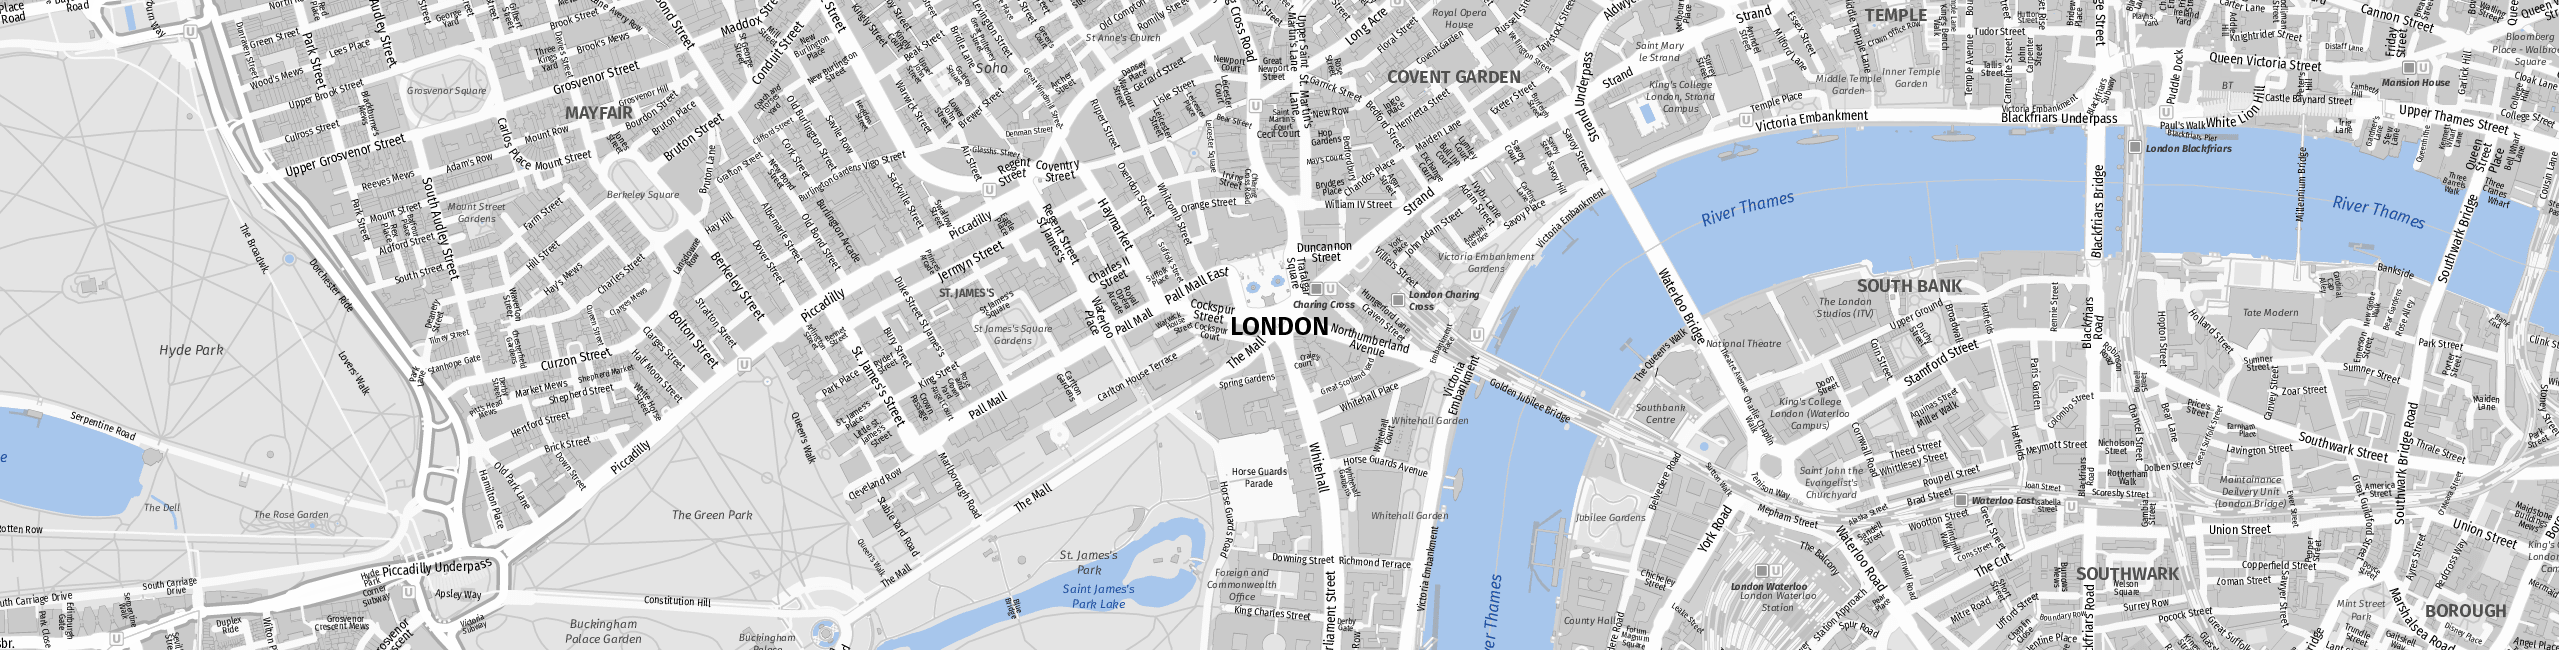
\includegraphics[height=\textheight,width=\textwidth,keepaspectratio]{map.png}
  \end{frame}

% ----------------------------------------- %

% Este efecto se ve muy bien pero es mas fastidioso de construir y modificar

  \begin{frame}
  \frametitle{A zoom over London}
  \begin{tikzpicture}[
  spy using outlines={
    circle,
    magnification=10,
    size=6cm,
    connect spies}]
  \node[inner sep=0pt] {\pgfimage[width=0.45\textwidth]{img/map.png}}; % Por algun motivo no reconoce la ubicacion por defecto
  \only<2>{\spy[red!70!black] on (0.5,0.15) in node at (.5\textwidth,0);}  % (0.5,0.15) es la porcion que se va a mostrar
  \end{tikzpicture}
  \end{frame}

% ----------------------------------------- %

  \begin{frame}{Frame Video}
    \begin{center}
    \movie[width=1\textwidth,showcontrols=true]
    {% placeholder = text or image
    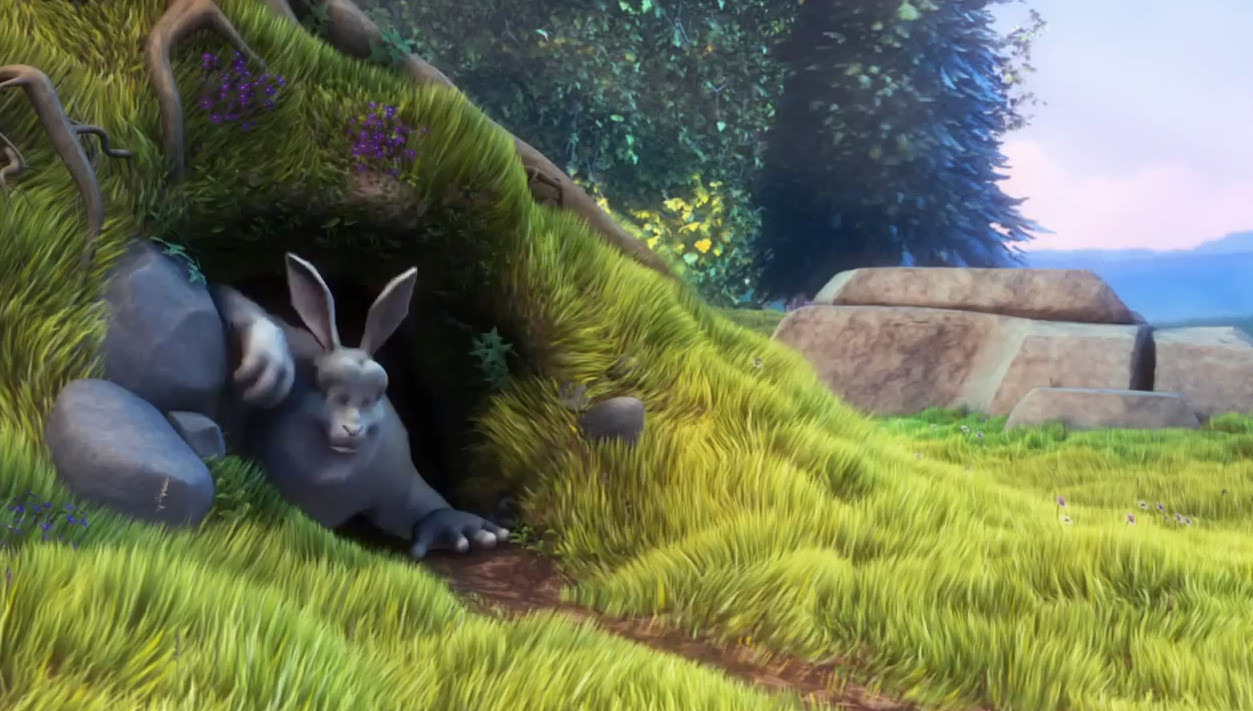
\includegraphics[width=1\textwidth]{thumbvideo.jpg}
    }%
    {media/sample.mp4} \\% video filename
    \end{center}
  \end{frame}

% ----------------------------------------- %

\end{document}
